\documentclass[aspectratio=43]{beamer}

% Pakete für das Dokument
\usepackage{blindtext}
\usepackage{todonotes}

\usepackage{../../inc/beamerthememnrstyle}

\usepackage{caption}
\usepackage{hyperref}
\captionsetup{justification   = raggedright,
              singlelinecheck = false}
% Eigenes Theme laden
\usetheme{mnrstyle}
\setbeamercovered { transparent }

% Eigene Definition von enumerate
% \setlist[enumerate, 2]{label=\roman*., format=\itshape, leftmargin=2cm}

% Metadaten für das Dokument
\title{Die Bibel}
\author{\MakeUppercase{Lothar Schmid}}
\date{2025}
\begin{document}

% Titelframe
\begin{frame}
    \maketitle    
\end{frame}
\begin{frame}
    \frametitle{Übersicht}  % Frametitel    
    \begin{enumerate}[<+->]        
        \item<1-> \only<1->{Ein Buch -- 2022 mehr als 35 Mio Bibeln} 
        
        \item<2-> \only<2->{Ein Buch -- mit 1200 - 1400 Seiten}   
        
        \item<3-> \only<3->{Ein Buch -- 2023 3686 Sprachen übersetzt\\
        (in 743 Sprachen die ganze Bibel)}                  
    \end{enumerate}   
\end{frame}

% Frametitel setzen
\begin{frame}
    \frametitle{Der Beginn}  % Frametitel
    \twocols[0.33]{
       \small Dieses Papyrusfragment von etwa 125 n. Chr. ist der älteste Beleg für das Neue Testament. Er handelt vom Prozess gegen Jesus: Die Frage »Bist du der König der Juden?« ist teilweise zu entziffern\\
    }[0.66]{
     \begin{figure}[t]
        \centering
        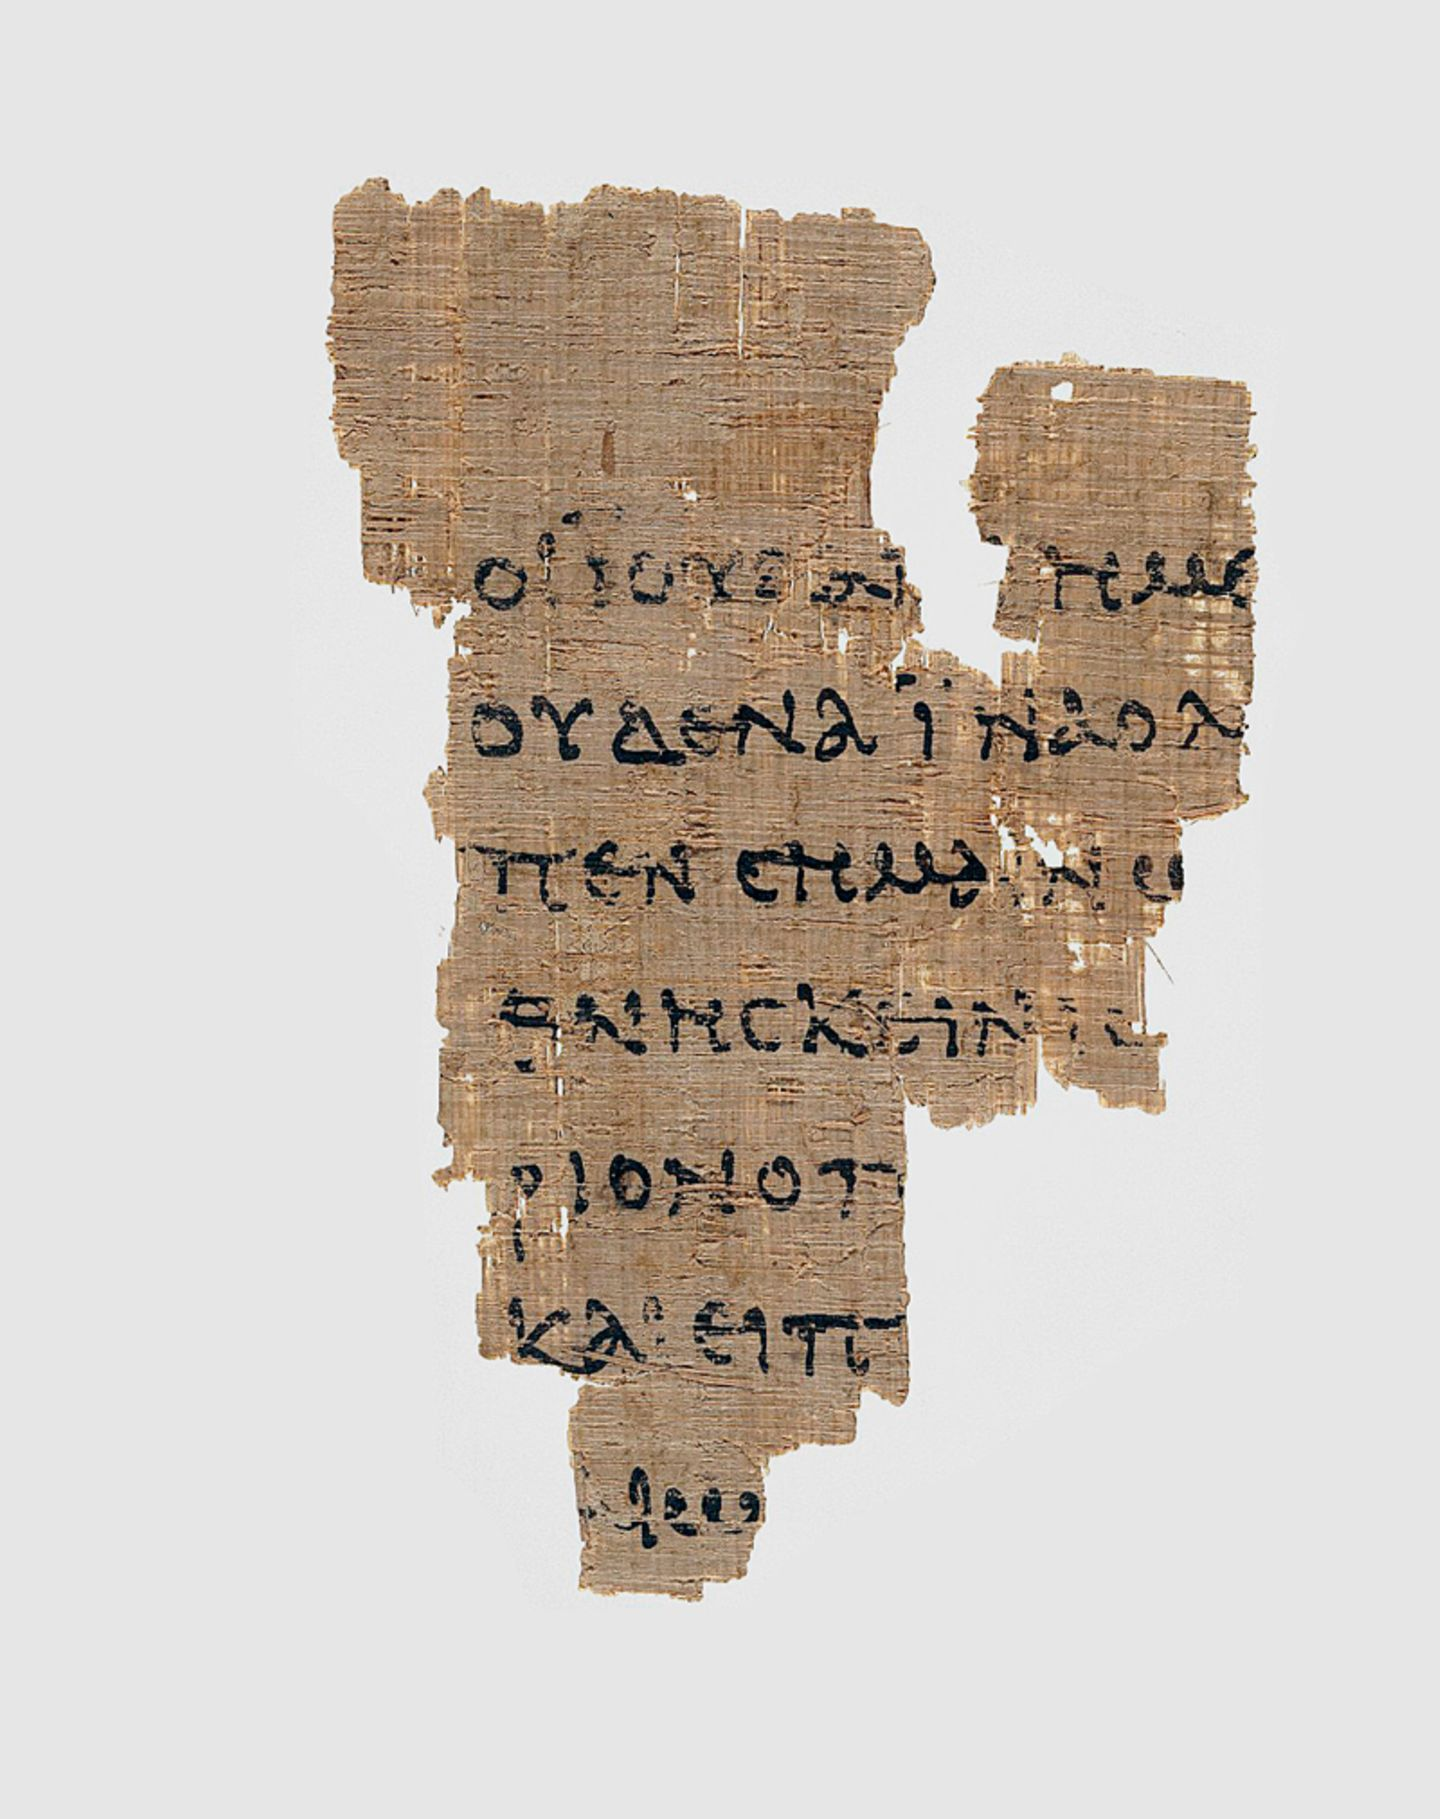
\includegraphics[width=0.5\linewidth]{src/Vorträge/BibelBuch/images/papyrusFragment.jpg}
        \caption{\centering \textcopyright John Rylands Library}
        \label{fig:enter-label}
    \end{figure}
    }    
\end{frame}
%%%%%%%%%%%%%%%%%%%%%%%%% Folie 3 %%%%%%%%%%%%%%%%%%%%%%%%%%%%%%%%
\begin{frame}
    \frametitle{Über Gott und den Menschen}  % Frametitel
    \begin{center}  
        \begin{tikzpicture}[overlay,remember picture]
            % \draw[gray!50!white,->] (current page.south west) grid[step=1mm] (current page.north east);
            \node[red,rotate=180,anchor=north west] at ([xshift=5cm,yshift=5cm]current page.south west) {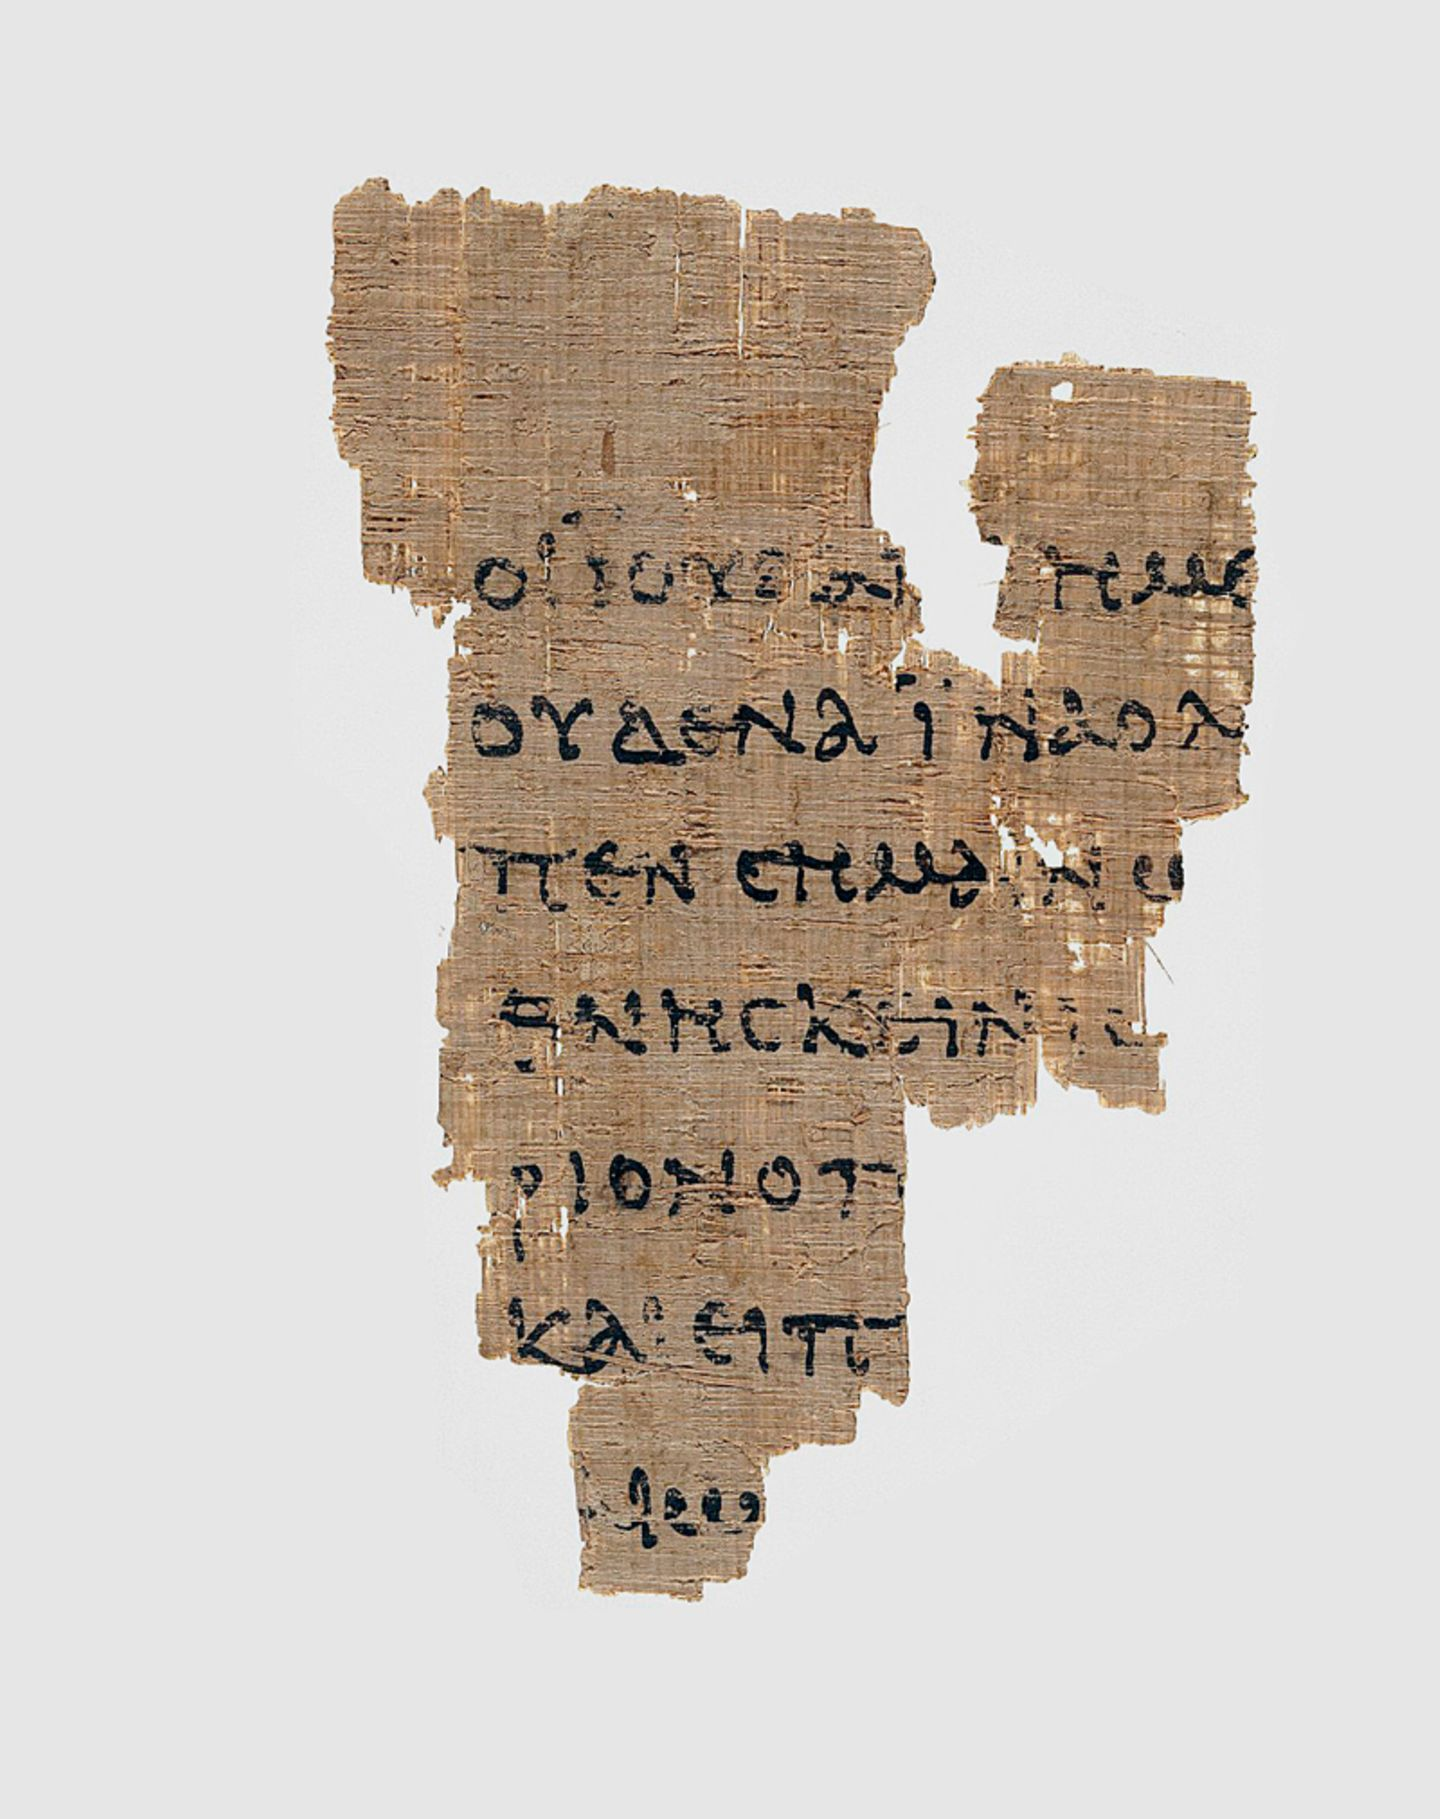
\includegraphics[width=2cm]{src/Vorträge/BibelBuch/images/papyrusFragment.jpg}};            
        \end{tikzpicture} 
            \captionof{figure}{Caption}
            \label{fig:enter-label}
    \end{center}
    \todo[inline]{Hier ein Todo}

    Hier ist ein anderer Text und der Text geht direkt weiter
\end{frame}

\end{document}
